\section{NFC Tag Data}
\label{sec:nfcdata}

The \ac{ndef} message stored on the \ac{nfc} tags for the application can contain the following three records and always in this order:

\begin{description}
\item[1. Exhibition ID] Contained in a text record. The exhibition ID is required for the user to register a user for the exhibition.
\item[2. Node ID] Contained in a text record and is used to show a specific node on the floor plan. The node ID is optional because we want the possibility for the user to just register for an exhibition without getting redirected to a node.
\item[3. Package name] Is an \ac{aar} and contains the unique package name for our application. When the Android platform reads an \ac{aar} it finds the application with that package name and launches it. If the application does not exist it sends the user to the Play Store where the application can be installed.
\end{description}
If the \ac{ndef} message contains both exhibition and node ID, then the exhibition ID should always come before the node ID.\autoref{fig:nfcdata} shows an example of an \ac{ndef} message for the application.

\begin{figure}[H]
\centering
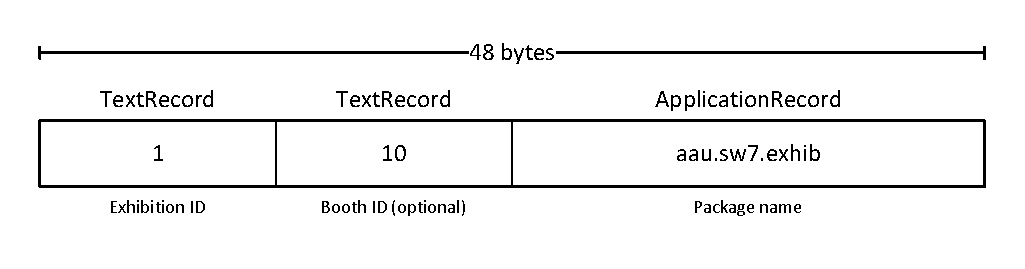
\includegraphics[width=0.97\columnwidth]{img/nfctag.pdf}
\caption{NFC tag message}
\label{fig:nfcdata}
\end{figure}
